\clearpage
\section{THE VOLUME ELEMENT}
Let $M$ be a $k$-dimensional manifold (or manifold-with-boundary) in $\F{R}^n$, 
with an orientation $\mu$. If $x\in M$, then $\mu_x$ and the inner product $T_x$ we defined 
previously determine a volume element $\omega(x) \in \Lambda^k(M_x)$. We therefore obtain a 
nowhere-zero $k$-form $\omega$ on $M$, which is called the \textbf{volume element}\index{Volume element}\indexsee{Element of volume}{Volume element} on $M$ 
(determined by $\mu$) and denoted $\dd V$, even though it is not generally the differential 
of a $(k-1)$-form. The \textbf{volume}\index{Volume} of $M$ is defined as $\int_M \;\dd V$, provided this integral 
exists, which is certainly the case if $M$ is compact. ``Volume'' is usually called \textbf{length}\index{Length} or 
\textbf{surface area}\index{Surface area}\index{Area!surface} for one- and two-dimensional manifolds, and $\dd V$ is denoted as 
(the ``element of length'')\index{Length!element of}\index{Element of area}\index{Area!element of}\index{Element of length} or 
$\dd A$ [or $\dd S$] (the ``element of [surface] area'').

A concrete case of interest to us is the volume element of an oriented \textbf{surface}\index{Surface}\index{Area!surface} 
(two-dimensional manifold) $M$ in $\F{R}^3$. Let $n(x)$ be the unit outward normal at
$x\in M$. If $\omega\in \Lambda^2(M_x)$ is defined by 
\begin{align*}
    \omega(v, w) = \det \begin{pmatrix}v\\ w\\ n(x)\end{pmatrix}
\end{align*} 

then $\omega(v,w)=1$ if $v$ and $w$ are an orthonomal basis of $M_x$ with $[v, w]=\mu_x$. 
Thus $\dd A=\omega$. On the other hand, $\omega(v, w)=\langle v\times w, n(x)\rangle$ by definition
of $v\times w$. Thus we have 
\begin{align*}
    \dd A(v, w) = \langle v\times w, n(x)\rangle
\end{align*}

Since $v\times w$ is a multiple of $n(x)$ for $v,w\in M_x$, we conclude that 
\begin{align*}
    \dd A(v, w) = |v\times w|
\end{align*} 

if $[v, w]=\mu_x$. If we wish to compute area of $M$, we must evaluate $\int_{[0,1]^2} c^*(\dd A)$ for 
orientation-preserving singular 2-cubes. Define 
\begin{align*}
    & E(a) = [\R{D}_1c^1(a)]^2 + [\R{D}_1c^2(a)]^2 + [\R{D}_1c^3(a)]^2\\
    & F(a) = [\R{D}_1c^1(a)]\cdot[\R{D}_2c^1(a)] \\
    & \hspace*{2.2em} + [\R{D}_1c^2(a)]\cdot[\R{D}_2c^2(a)] + [\R{D}_1c^3(a)]\cdot[\R{D}_2c^3(a)]\\
    & G(a) = [\R{D}_2c^1(a)]^2 + [\R{D}_2c^2(a)]^2 + [\R{D}_2c^3(a)]^2
\end{align*}

Then 
\begin{align*}
    & c^*(\dd A)((e_1)_a, (e_2)_a) = \dd A(c_*(e_1)_a, c_*(e_2)_a) \\
    & = |(\R{D}_1c^1(a), \R{D}_1c^2(a), \R{D}_1c^3(a)) \times (\R{D}_2c^1(a), \R{D}_2c^2(a), \R{D}_2c^3(a))| \\
    & = \sqrt{E(a)G(a) - F(a)^2}
\end{align*}

by Problem 4-9. Thus 
\begin{align*}
    \int_{[0,1]^2} c^*(\dd A) = \int_{[0,1]^2} \sqrt{EG-F^2}
\end{align*}

Calculating surface area is clearly a foolhardy enterprise;
fortunately one seldom needs to know the \textbf{area}\index{Surface area} of a surface.
Moreover, there is a simple expression for $\dd A$ which suffices for
theoretical considerations.

\begin{theorem}
    Let $M$ be an oriented two-dimensional manifold (or manifold-with-boundary) in $\F{R}^3$ 
    and let n be the unit outward normal. Then
    \begin{align}
        \dd A=n^1\dd y\wedge\dd z+n^2\dd z\wedge\dd x+n^3\dd x\wedge\dd y.
    \end{align}

    Moreover 
    \begin{align}
        n^1\dd A & = \dd y\wedge \dd z\\
        n^2\dd A & = \dd z\wedge \dd x\\
        n^3\dd A & = \dd x\wedge \dd y
    \end{align}
\end{theorem}

\begin{proof}
    Equation (1) is equivalent to the equation
    \begin{align*}
        \dd A(v, w) = \det 
        \begin{pmatrix}
            v\\ w\\ n(x)
        \end{pmatrix}
    \end{align*}

    This is seen by expanding the determinant by minors along the bottom row.
    To prove the other equations, let $z\in\F{R}^3_x$. Since $v\times w=\alpha n(x)$ for some 
    $\alpha\in\F{R}$, we have 
    \begin{align*}
        \langle z, n(x)\rangle\cdot \langle v\times w, n(x)\rangle
        & = \langle z, n(x)\rangle\alpha 
        & = \langle z, \alpha n(x)\rangle
        & = \langle z, v\times w\rangle
    \end{align*}

    Choosing $z=e_1, e_2$, and $e_3$ we obtain (2), (3), and (4).
\end{proof}


A word of caution: if $\omega\in \Lambda^2(\F{R}^3_a)$ is defined by 
\begin{align*}
    \omega
    = n^1(a)\cdot \dd y(a)\wedge\dd z(a)
    + n^{2}(a)\cdot\dd z(a)\wedge\dd x(a)
    + n^{3}(a)\cdot\dd x(a)\wedge\dd y(a)
\end{align*}

it is not true, for example, that
\begin{align*}
    n^1(a)\cdot\omega = \dd y(a)\wedge\dd z(a)
\end{align*}

\begin{figure}[!htb]
    \centering
    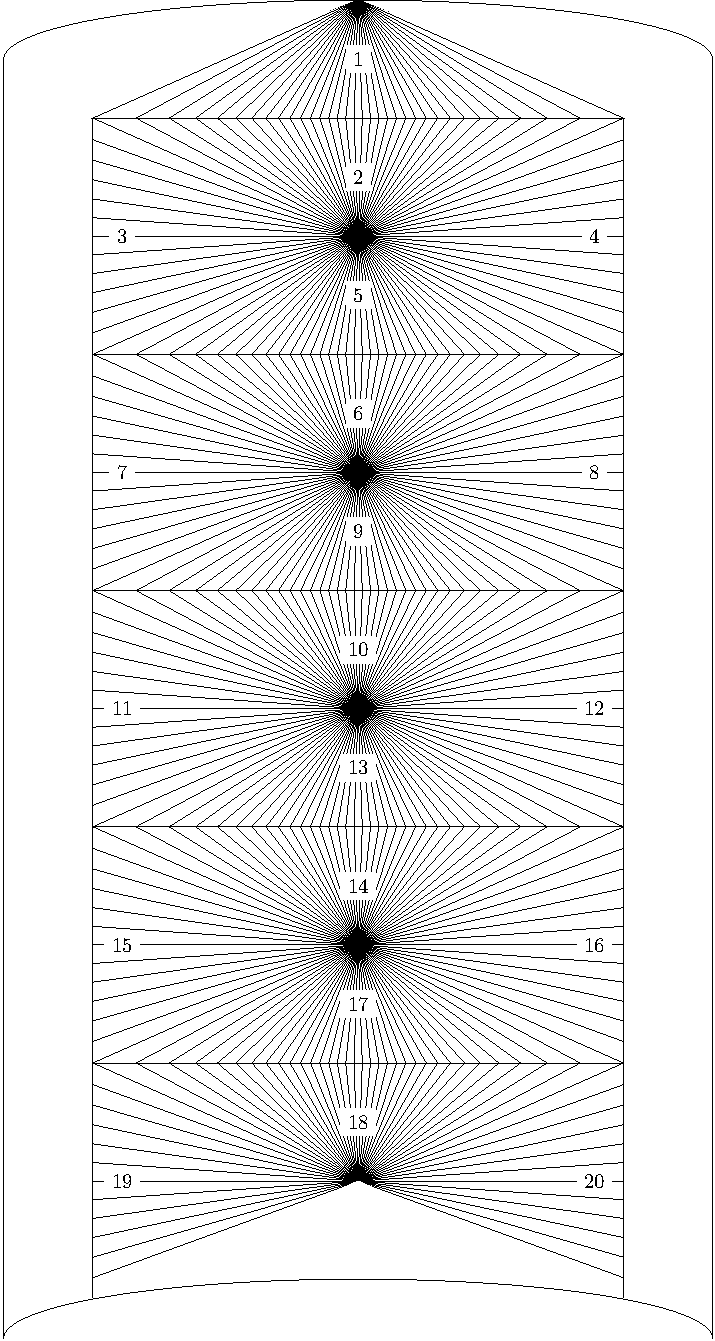
\includegraphics[width=.75\linewidth]{./pics/Fig5-9.pdf}
    \caption{\textit{A surface containing 20 triangles inscribed in a portion of a cylinder. 
    If the number of triangles is increased sufficiently, by making the bases of triangles 
    3, 4, 7, 8, etc., sufficiently small, the total area of the inscribed surface can be made as 
    large as desired.}}
    \label{Fig 5-9}
\end{figure}

A few remarks should be made to justify the definition of
length and surface area we have given. If $c:[0,1]\to \F{R}^n$ is
differentiable and $c([0,1])$ is a one-dimensional manifold-with-
boundary, it can be shown, but the proof is messy, that the
length of $c([0,1])$ is indeed the least upper bound of the lengths
of inscribed broken lines. If $c:[0,1]^2\to \F{R}^n$, one naturally
hopes that the area of $c([0,1]^2)$ will be the least upper bound of
the areas of surfaces made up of triangles whose vertices lie in
$c([0,1]^2)$. Amazingly enough, such a least upper bound is
usually nonexistent-one can find inscribed polygonal surfaces
arbitrarily close to $c([0,1]^2)$ with arbitrarily large area! This
is indicated for a cylinder in Figure \ref{Fig 5-9}. Many definitions
of surface area have been proposed, disagreeing with each
other, but all agreeing with our definition for differentiable
surfaces. For a discussion of these difficult questions the
reader is referred to References \cite{cesari1956surface} or \cite{rad61948length}.

\begin{problems}
    \problem{
        If $M$ is an oriented one-dimensional manifold in $\F{R}^n$ and $c:[0,1]\to M$ is 
        orientation-preserving, show that
        \begin{align*}
            \int_{[0,1]}c^*(\dd s)
            = \int_{[0,1]}\sqrt{[(c^1)']^2 + \cdots + [(c^n)']^2}
        \end{align*}
    }
    \problem{
        If $M$ is an $n$-dimensional manifold in $\F{R}^n$, with the usual orientation, 
        show that $\dd V=\dd x^1\wedge\cdots\wedge\dd x^n$, so that the volume of
        $M$, as defined in this section, is the volume as defined in Chapter 3.
        (Note that this depends on the numerical factor in the definition of $\omega\wedge\eta$)
    }
    \problem{
        Generalize Theorem 5-6 to the case of an oriented $(n-1)$-dimensional manifold in $\F{R}^n$.
    }
    \problem{
        \begin{enumerate}[label=(\alph*)]
            \item If $f: [a,b]\to \F{R}$ is non-negative and the graph of $f$ in the
                $xy$-plane is revolved around the $x$-axis in $\F{R}^3$ to yield a surface $M$,
                show that the area of $M$ is
                \begin{align*}
                    \int_a^b 2\pi f\sqrt{1+(f')^2}
                \end{align*}
            \item Compute the area of $S^2$.
        \end{enumerate}
    }
    \problem{
        If $T:\F{R}^n\to\F{R}^n$ is a norm preserving linear transformation and $M$
        is a $k$-dimensional manifold in $\F{R}^n$, show that $M$ has the same
        volume as $T(M)$.
    }
    \problem{
        \begin{enumerate}[label=(\alph*)]
            \item If $M$ is a $k$-dimensional manifold, show that an absolute
                $k$-tensor $|\dd V|$ can be defined, even if $M$ is not orientable, so that
                the volume of $M$ can be defined as $\int_M |\dd V|$.
            \item If $c:[0, 2\pi]\times (-1, 1)\to \F{R}^3$ is defined by $c(u,v) = (2\cos u + v\sin(u/2)\cos u, 2\sin u+ v\sin(v/2)\sin u, v\cos u/2)$,
                show that $c([0, 2\pi]\times(-1,1))$ is a M\"obius strip\index{M\"obius strip} and find its erea.
        \end{enumerate}
    }
    \problem{
        If there is a nowhere-zero $k$-form on a $k$-dimensional manifold $M$, show that $M$ is orientable.
    }
    \problem{
        \begin{enumerate}[label=(\alph*)]
            \item If $f:[0,1]\to \F{R}$ is differentiable and $c:[0,1]\to \F{R}^2$ is defined
                by $c(x)=(x, f(x))$, show that $c([0,1])$ has length $\int_{[0,1]}\sqrt{1+(f')^2}$.
            \item Show that this lenght is the least upper bound of lengths of inscribed lines. \textit{Hint:}
                If $0=t_0\le t_1\le\cdots\le t_n=1$, then 
                \begin{align*}
                    \left|c(t_i)-c(t_{i-1})\right|
                    & = \sqrt{\left(t_i-t_{i-1}\right)^2+\left(f(t_i)-f(t_{i-1})\right)^2} \\
                    & = \sqrt{\left(t_i-t_{i-1}\right)^2+f'(s_i)^2\left(t_i - t_{i-1}\right)^2}
                \end{align*}

                for some $s_i\in [t_{i-1}, t_i]$.
        \end{enumerate}
    }
    \problem{
        Consider the 2-form $\omega$ defined on $\F{R}^3-\{0\}$ by
        \begin{align*}
            \omega=\frac{x\dd y\wedge\dd z+y\dd z\wedge\dd x+z\dd x\wedge\dd y}{(x^2+y^2+z^2)^{\frac32}} 
        \end{align*}
        \begin{enumerate}[label=(\alph*)]
            \item Show that $\omega$ is closed.
            \item Show that 
                \begin{align*}
                    \omega(p)(v_p, w_p) = \frac{\langle v\times w, p\rangle}{|p|^3}
                \end{align*}

                For $r>0$ let $S^2(r)=\{x\in\F{R}^3:|x|=r\}$. Show that $\omega$ restricted to the  
                tangent space of $S^2(r)$ is $1/r^2$ times the volume element, and that $\int_{S^2(r)}\omega=4\pi$.
                Conclude that $\omega$ is not exact. Nevertheless we denoted $\omega$ by $\dd\Theta$ since, as we 
                shall see, $\dd\Theta$ is the analogue of the 1-form $\dd\theta$ on $\F{R}^2-\{0\}$.
            \item If $v_p$ is a tangent vector such that $v=\lambda_p$ for some $\lambda\in\F{R}$, show that 
                $\dd\Theta(p)(v_p,w_p)=0$ for all $w_p$. If a two-dimensional manifold $M$ in $\F{R}^3$ is
                part of a \textbf{generalized cone}\index{Generalized cone}\index{Cone, generalized}, that is, $M$ is the union of segment of rays through the origin, show
                that $\int_M\dd\Theta =0$. 
            \item Let $M\subset\F{R}^3-\{0\}$ be a compact two-dimensional manifold-with-boundary 
                such that every ray through 0 intersects Mat most once (Figure 5-10).
                The union of those rays through 0 which intersect $M$, is a solid cone $C(M)$. 
                The \textbf{solid angle}\index{Solid angle}\Index{Angle!solid} subtended by $M$ is defined as the area of $C(M)\cap S^2$, or 
                equivalently as $1/r^2$ times the area of $C(M)\cap S^2(r)$ for $r > 0$.
                Prove that the solid angle subtended by $M$ is $|\int_M\dd\Theta|$.
                \textit{Hint}: Choose $r$ small enough so that there is a three-dimensional 
                manifold-with-boundary $N$ (as in Figure \ref{Fig 5-10}) such that $\partial N$ is the 
                union of $M$ and $C(M)\cap S^2(r)$, and a part of a generalized cone.(Actually, $N$ 
                will be a \textbf{manifold-with-corners}\index{Manifold-with-corners}; see the remarks at the end of the next section.)

                % \begin{figure}[htb]
                %     \centering
                %     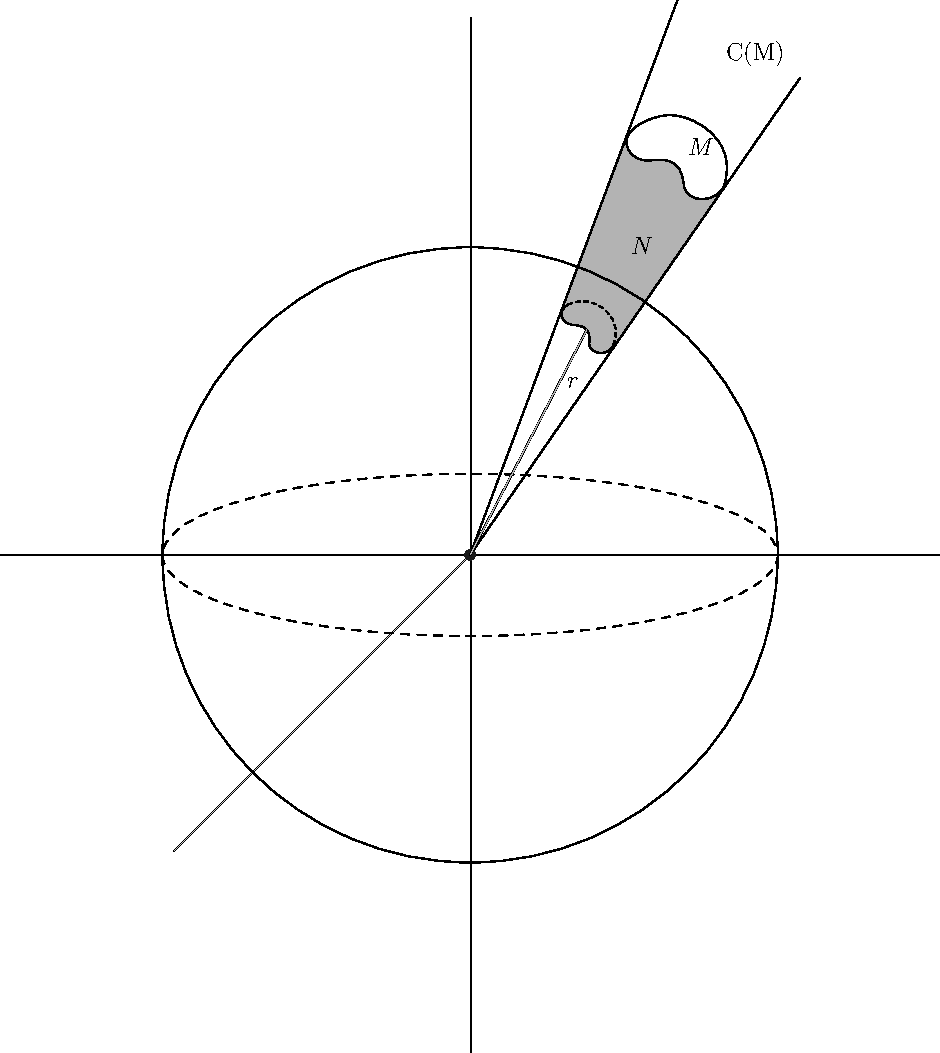
\includegraphics[width=.75\linewidth]{./pics/Fig5-10.pdf}
                %     \caption{}
                %     \label{Fig 5-10}
                % \end{figure}
        \end{enumerate}
    }
    \problem{
        Let $f,g:[0,1]\to\F{R}^3$ be the nonintersecting closed curves. Define the \textbf{linking number}\index{Linking number} 
        $l(f,g)$ of $f$ and $g$ be (cf Problem 4-34)
        \begin{align*}
            l(f,g) = \frac{-1}{4\pi}\int_{c_{f,g}}\dd\Theta
        \end{align*}
        \begin{enumerate}[label=(\alph*)]
            \item Show that if $(F,G)$ is a homotopy of nonintersecting closed curves, then 
                $l(F_0,G_0) = l(F_1,G_1)$.
            \item If $r(u,v)=|f(u)-g(v)|$ show that 
                \begin{align*}
                    l(f,g)=\frac{-1}{4\pi}\int_{0}^{1}\int_{0}^{1}\frac{1}{[r(u,v)]^3}\cdot A\left(u,v\right)\;\dd u\dd v
                \end{align*}

                where 
                \begin{align*}
                    A(u,v)=\det
                    \begin{pmatrix}
                        (f^1)^{\prime}(u)&(f^2)^{\prime}(u)&(f^3)^{\prime}(u)\\
                        (g^1)^{\prime}(v)&(g^2)^{\prime}(v)&(g^3)^{\prime}(v)\\
                        f^1(u)-g^1(v)&f^2(u)-g^2(v)&f^3(u)-g^3(v)
                    \end{pmatrix}.
                \end{align*}
            \item Show that $l(f,g) = 0$ if $f$ and $g$ both lie in the $xy$-plane.
                The curves of Figure 4-5 (b) are given by $f(u) = (\cos u, \sin u, 0)$
                and $g(v) = (1 +\cos v, 0, \sin v)$. You may easily convince yourself that 
                calculating $l(f,g)$ by the above integral is hopeless in this case. 
                The following problem shows how to find $l(f,g)$ without explicit calculations.
        \end{enumerate}
    }
    \problem{
        \begin{enumerate}[label=(\alph*)]
            \item If $(a,b,c)\in\F{R}^3$ define 
                \begin{align*}
                    \dd\Theta_{(a,b,c)}=\frac{(x-a)\dd y\wedge\dd z+(y-b)\dd z\wedge\dd x+(z-c)\dd x\wedge\dd y}{[(x-a)^2+(y-b)^2+(z-c)^2]^\frac32}
                \end{align*}

                If $M$ is a compact two-dimensional manifold-with-boundary in $\F{R}^3$ and $(a,b,c)\notin M$ 
                define
                \begin{align*}
                    \Omega(a,b,c)=\int_{M}\;\dd\Theta_{(a,b,c)}.
                \end{align*}

                Let $(a',b',c')$ be a point on the same side of $M$ as the outward normal and $(a',b'c')$
                a point on the oppsite side. Show that by choosing $(a,b,c)$ sufficently close to $(a'.b',c')$ we can 
                make $\Omega(a,b,c)-\Omega(a',b',c')$ as close to $-4\pi$ as desired. \textit{Hint:} First 
                show that if $M=\partial N$ then $\Omega(a,b,c)=-4\pi$ for $(a,b,c)\in N-M$ and $\Omega(a,b,c)=0$
                for $(a,b,c)\notin N$.
            \item Suppose $f([0,1]) = \partial M$ for some compact oriented two-dimensional 
                manifold-with-boundary $M$. (If $f$ does not intersect itself such an $M$ always 
                exists, even if $f$ is knotted, see [6], page 138.) Suppose that whenever $g$ 
                intersects $M$ at $x$ the tangent vector $v$ of $g$ is not in $M_x$·
                Let $n^+$ be the number of intersections where $v$ points in the same direction as 
                the outward normal and $n^-$ the number of other intersections. If $n=n^+ - n^-$ show that
                \begin{align*}
                    n=\frac{-1}{4\pi}\int_{g}\;\dd\Omega
                \end{align*}
            \item Prove that 
                \begin{align*}
                    \R{D}_{1}\Omega(a,b,c) & = \int_{f}\frac{(y-b)\dd z-(z-c)\dd y}{r^{3}} \\
                    \R{D}_{2}\Omega(a,b,c) & = \int_{f}\frac{(z-c)\dd x-(x-a)\dd z}{r^{3}} \\
                    \R{D}_{3}\Omega(a,b,c) & = \int_{f}\frac{(x-a)\dd y-(y-b)\dd x}{r^{3}}
                \end{align*}

                where $r(x,y,z)=|(x,y,z)|$.
            \item Show that the integer $n$ of (b) equals the integral of Problem 5-32(b), 
                and use this result to show that $l(j,g) = 1$ if $f$ and $g$ are the curves 
                of Figure 4-6 (b), while $l(f,g) = 0$ if $f$ and $g$ are the curves of Figure 4-6 (c). 
                (These results were known to Gauss\index{Gauss} \cite{gaussNachlass}. The proofs outlined here 
                are from \cite{courant1937differential} pp. 409-411; see also \cite{maxwell1954electricity}, 
                Volume 2, pp. 41-43.)
                \begin{figure}[H]
                    \centering
                    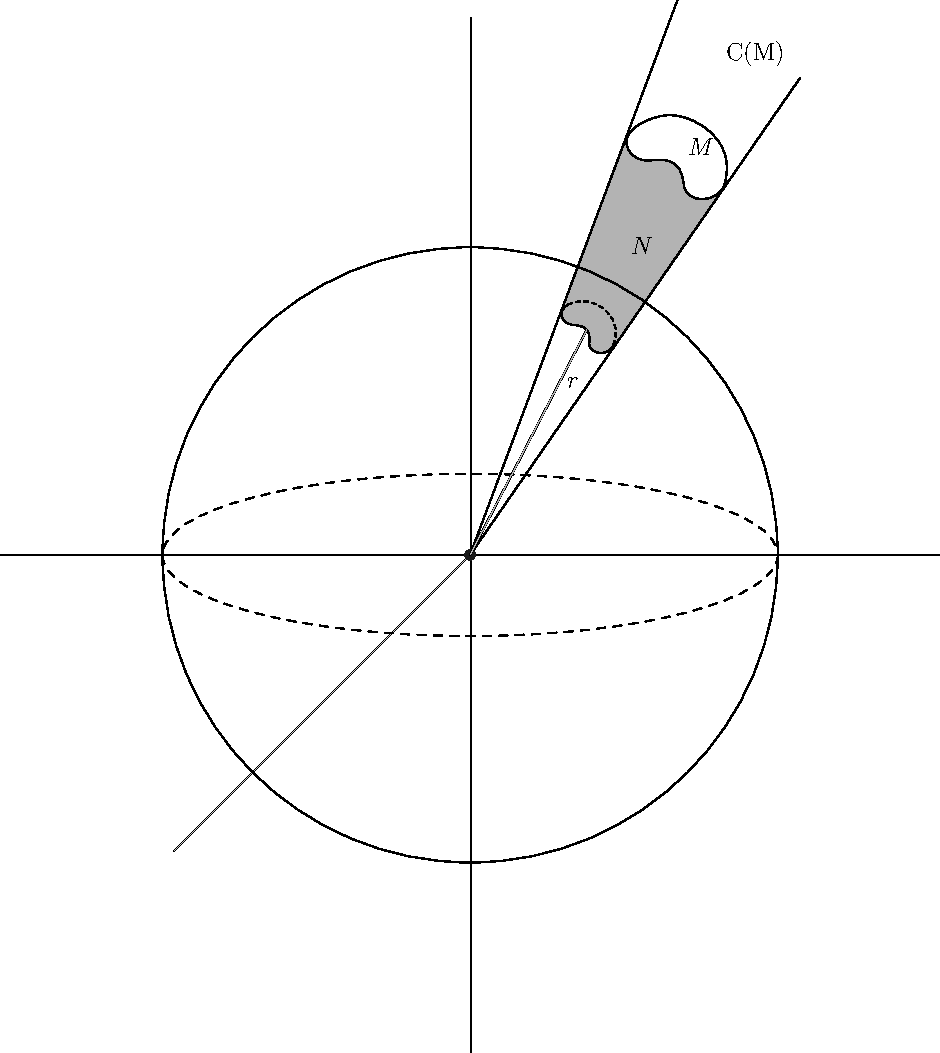
\includegraphics[width=.65\linewidth]{./pics/Fig5-10.pdf}
                    \caption{}
                    \label{Fig 5-10}
                \end{figure}
        \end{enumerate}
    }
\end{problems}